\documentclass[xcolor={table}]{beamer}
\usepackage[english]{babel}
\usepackage[utf8]{inputenc}

\usepackage{hyperref}
\usepackage{url}
\usepackage{amsmath}
\usepackage{graphicx}
\usepackage{animate}
\usepackage{enumerate}
\usepackage{subcaption}
\usepackage{multicol}
\usepackage[full, italic, slant]{complexity}
\usepackage{appendixnumberbeamer}


\expandafter\def\expandafter\insertshorttitle\expandafter{%
  \insertshorttitle\hfill\insertframenumber\,/\,\inserttotalframenumber}

\def\*{{\bf FIXME: }}

\setbeamertemplate{caption}[numbered]
\setbeamertemplate{bibliography item}{\insertbiblabel}
\newtheorem{deff}{Definícia}[section]

\mode<presentation> {
    \usetheme{Warsaw}
    \usecolortheme{seahorse}
    \usecolortheme{rose}
    \usefonttheme{professionalfonts}
    \setbeamercovered{transparent}
}

\definecolor{bloodred}{RGB}{200,0,0}


\title{Improving LSA word weights for document classification}
\author{Bc. Vladimír Macko}
\institute{RNDr. Kristína Malinovská, PhD.}



\begin{document}
        
\begin{frame}
    \titlepage
\end{frame}
    
\begin{frame}{Overview}
    \begin{block}{}
        \begin{itemize}
            \item Introduction
            \item Problem outline
            \item Our work
            \item Results
        \end{itemize}
    \end{block}
\end{frame}

%%%%%%%%%%%%%%%%%%%%%
\section{Introduction}
\begin{frame}{Document classification}
    \begin{block}{}
        \emph{This was a terrible movie}
    \end{block}
    
    \begin{block}{}   
        \begin{itemize}
            \item create representation for words
            \item create representation for document
            \item predict
            \item small, specific datasets
        \end{itemize}
    \end{block}
\end{frame} 

\begin{frame}{Word vectors}
    \begin{columns}
       \column{0.5\linewidth}
        Local representation
        
        $[0,0,1,0,0]$
        \begin{block}{}
            One hot encoding
        \end{block}

        \column{0.5\linewidth}
        Distributed representation
        $[0.1,0.2,0.6,0.05,0.05]$
        \begin{block}{Count based}
            Factorization of co-occurrence matrix
            
            LSA (SVD)
        \end{block}
        \begin{block}{Prediction based}
            Trained neural network

            Skip gram    
        \end{block}    
   \end{columns}
\end{frame} 

\begin{frame}{LSA}
~
    {\tiny $$
\begin{matrix} 
 M &  ~~ U & \Sigma & V^T \\
 \textbf{t}_j^T &  & &  \\
 \downarrow &  & &  \\
(\textbf{d}_i) \rightarrow 
\begin{bmatrix}
x_{1,1} \dots  x_{1,n} \\
\vdots ~~~  \ddots ~~~ \vdots \\
x_{i,1} \dots  x_{i,n} \\
\vdots ~~~ \ddots ~~~ \vdots \\
x_{m,1} \dots  x_{m,n} \\
\end{bmatrix}
=
&
\textbf{u}_i \rightarrow
\begin{bmatrix} 
\begin{bmatrix} & \textbf{u}_1 & \end{bmatrix} \\
\vdots \\
\begin{bmatrix} & \textbf{u}_m & \end{bmatrix}
\end{bmatrix}
&
\cdot
\begin{bmatrix} 
\sigma_1 \dots ~~~ 0 \\
\vdots ~~~ \ddots  \vdots \\
0  \dots  \sigma_l \\
\end{bmatrix}
&
\cdot
\begin{bmatrix} 
\begin{bmatrix} \, \\ \, \\ \textbf{v}_1 \\ \, \\ \,\end{bmatrix} 
\dots
\begin{bmatrix} \, \\ \, \\ \textbf{v}_n \\ \, \\ \, \end{bmatrix}
\end{bmatrix}
\end{matrix}
$$}
    \begin{block}
        
        $d_i$: bag of words
        
        $u_i$: word vector
        
        $M$: co-occurrence matrix
        
        $v_i$: document vector
        
        $d_i U$: lower dimensional embedding $\rightarrow$ train classifier
    \end{block}
\end{frame}

%%%%%%%%%%%%%%%%%%%%%%%%%
\section{Problem outline}
\begin{frame}{LSA problems}
    \begin{block}{}
        \begin{itemize}
            \item Most representative features, not most discriminative
            \item Sensitive to preprocessing
            \item Sensitive to weights
            \item Unsupervised and can forget things
        \end{itemize}
    \end{block}
\end{frame} 

\begin{frame}{Current solutions}
    $$ d_i \rightarrow_w \hat{d_i} $$
    
    Factorize $M$ train classifier on low dimensionality embeddings

    \begin{block}{}
        \begin{itemize}
            \item Preprocessing
            \item Weight - Mutual information \cite{wu2017balancing}, \cite{deng2014study}
            \item Supervised weights: TF-KLD \cite{ji2013discriminative}, \cite{lan2009supervised}
        \end{itemize}
    \end{block}
\end{frame} 


\section{Our work}
\begin{frame}{Our system}
    \begin{block}{Baseline}
        \begin{itemize}
            \item Apply weighting scheme $w$, factorize, predict 
            \item Training the predictor
        \end{itemize}
    \end{block}

    \begin{block}{Our approach}
        \begin{itemize}
            
            \item Apply weighting scheme $w$, rescale with $w'$, factorize, predict 
            \item Training the predictor, optimize $w'$
        \end{itemize}
    \end{block}
    
    LSA used in similar manner in \cite{ionescu2015training}
\end{frame} 

\begin{frame}{Gradient descent}
    \begin{columns}    
    \column{0.5\linewidth}
    \begin{itemize}
        \item Co-occurrence matrix $M$
        \item Weight vector $w'$
    \end{itemize}
    \column{0.5\linewidth}
    \begin{itemize}
        \item SVD: $U \Sigma V^T$
        \item Simple classifier: $\sigma (v \theta + b)$
    \end{itemize}    
    \end{columns}

    \begin{block}{}
    \begin{itemize}
        \item Reweighted matrix $M \circ w'$
        \item SVD decomposition $M \circ w' = U \Sigma V^T$
        \item Compute embedding $v = d \circ w' U$
        \item Train classifier $\hat{y} = \sigma (v \theta + b)$ to minimize $E = \frac{1}{2}(\hat{y}-y)^2$
        \item Compute derivative $\frac{\partial E}{\partial w'} = (\hat{y} -y) \hat{y} (1-\hat{y})\Theta U$
        \item Update weights: $w' = w' - \alpha \frac{\partial E}{\partial w'}$
    \end{itemize}    
    \end{block}
\end{frame} 

\begin{frame}{Evaluation}
    \begin{block}{Datasets from SentEval \cite{conneau2017supervised}}
        \begin{itemize}
            \item Customer review dataset
            \item Movie review
            \item Subjective vs objective
            \item Opinion polarity            
        \end{itemize}
    \end{block}
    
    
\end{frame} 

\section{Results}

\begin{frame}{Baseline on customer review dataset}
    \begin{columns}
        \column{0.5\linewidth}
                   \begin{figure}[H]
                    \centering
                    \caption*{SVD + logistic regression}
                    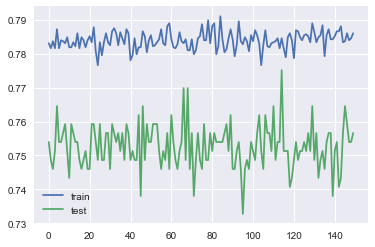
\includegraphics[height=0.4\textheight]{images/CRDataset.png}
                    \caption{Precision of baseline on CR dataset for multiple tries}
                \end{figure}
            \column{0.5\linewidth}

                \begin{figure}[H]
                    \centering
                    \caption*{TFIDF + SVD + logistic regression}
                    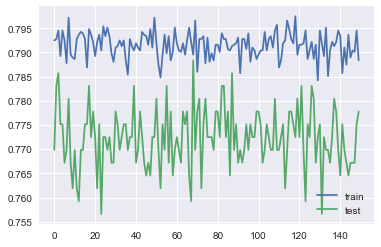
\includegraphics[height=0.4\textheight]{images/CRDataset_tfidf.png}
                    \caption{Precision of baseline on CR dataset for multiple tries}
                \end{figure}
    \end{columns}
                
\end{frame} 

\begin{frame}{Our method on customer review dataset}
    \begin{columns}
        \column{0.5\linewidth}
                   \begin{figure}[H]
                    \centering
                    \caption*{SVD + LR + gradient}
                    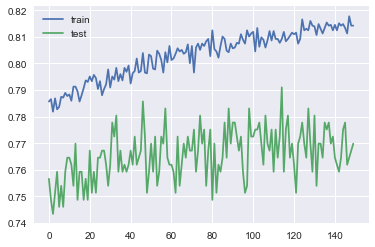
\includegraphics[height=0.4\textheight]{images/CRDataset_grad.png}
                    \caption{Precision of weight improving on CR dataset for multiple epochs}
                \end{figure}
            \column{0.5\linewidth}

                \begin{figure}[H]
                    \centering
                    \caption*{TFIDF + SVD + LR + gradient}
                    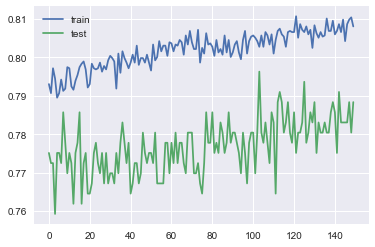
\includegraphics[height=0.4\textheight]{images/CRDataset_tfidf_grad.png}
                    \caption{Precision of tfidf weight improving on CR dataset for multiple epochs}
                \end{figure}
    \end{columns}                
\end{frame} 

\begin{frame}[fragile]{Insight}
    \begin{columns}
        \column{0.25\linewidth}
        	$w'$ 
\begin{verbatim}
1.55: 't
1.38: slow
1.37: plus
1.34: good
1.34: flaw
1.33: bit
1.33: perfect
1.31: excellent
1.29: the
1.27: to
\end{verbatim}
        \column{0.25\linewidth}
\begin{verbatim}
0.20: i
0.56: diaper
0.56: camera
0.57: and
0.60: 3
0.61: am
0.63: small
0.64: !
0.69: very
0.71: does
\end{verbatim}
        \column{0.25\linewidth}
        $w'$ for TFIDF
\begin{verbatim}
1.72: not
1.67: only
1.49: great
1.41: 't
1.37: easy
1.28: good
1.26: after
1.23: but
1.23: excellent
1.19: bit
\end{verbatim}
        \column{0.25\linewidth}
\begin{verbatim}
0.91: ,
0.92: is
0.93: for
0.95: this
0.95: it
0.96: has
0.97: very
0.97: screen
0.98: say
0.98: antivirus
\end{verbatim}
    \end{columns}
\end{frame}

\begin{frame}{Our method on movie review dataset}
    \begin{columns}
        \column{0.5\linewidth}
                   \begin{figure}[H]
                    \centering
                    \caption*{SVD + LR + gradient}
                    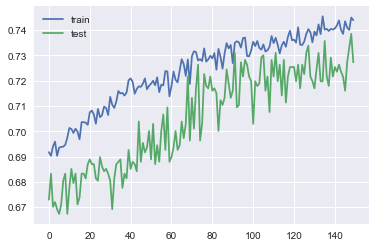
\includegraphics[height=0.4\textheight]{images/MRDataset_grad.png}
                    \caption{Precision of weight improving on MR dataset for multiple epochs}
                \end{figure}
            \column{0.5\linewidth}

                \begin{figure}[H]
                    \centering
                    \caption*{TFIDF + SVD + LR + gradient}
                    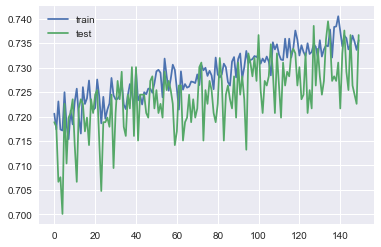
\includegraphics[height=0.4\textheight]{images/MRDataset_tfidf_grad.png}
                    \caption{Precision of tfidf weight improving on MR dataset for multiple epochs}
                \end{figure}
    \end{columns}                
\end{frame} 

\begin{frame}{Our method on opinion polarity review dataset}
    \begin{columns}
        \column{0.5\linewidth}
            \begin{figure}[H]
                \centering
                \caption*{SVD + LR + gradient}
                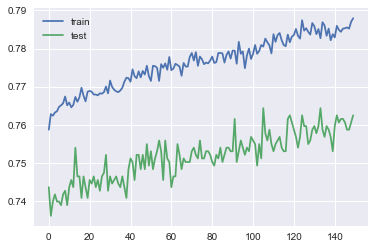
\includegraphics[height=0.4\textheight]{images/MPQADataset_grad.png}
                \caption{Precision of weight improving on MPQA dataset for multiple epochs}
            \end{figure}
        \column{0.5\linewidth}

            \begin{figure}[H]
                \centering
                \caption*{TFIDF + SVD + LR + gradient}
                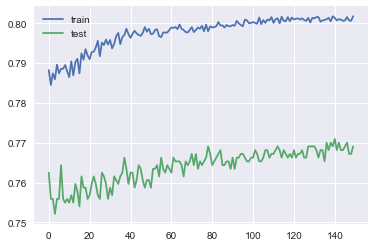
\includegraphics[height=0.4\textheight]{images/MPQADataset_tfidf_grad.png}
                \caption{Precision of tfidf weight improving on MPQA dataset for multiple epochs}
            \end{figure}
    \end{columns}                
\end{frame} 

\begin{frame}{Our method on subjective/objective dataset}
    \begin{columns}
        \column{0.5\linewidth}
                   \begin{figure}[H]
                    \centering
                    \caption*{SVD + LR + gradient}
                    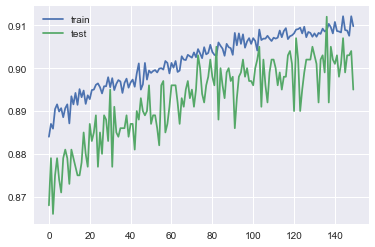
\includegraphics[height=0.4\textheight]{images/SUBJDataset_grad.png}
                    \caption{Precision of weight improving on SUBJ dataset for multiple epochs}
                \end{figure}
            \column{0.5\linewidth}

                \begin{figure}[H]
                    \centering
                    \caption*{TFIDF + SVD + LR + gradient}
                    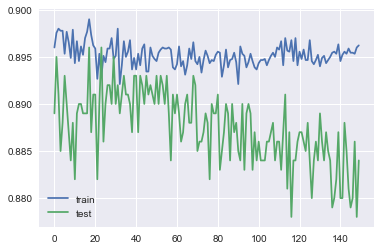
\includegraphics[height=0.4\textheight]{images/SUBJDataset_tfidf_grad.png}
                    \caption{Precision of tfidf weight improving on SUBJ dataset for multiple epochs}
                \end{figure}
    \end{columns}                
\end{frame} 



\begin{frame}{Plans}
    \begin{block}{}
        \begin{itemize}   
            \item Try other weight schemes
            \item Compare to word2vec
            \item More datasets 
        \end{itemize}
    \end{block}
\end{frame} 


\begin{frame}
    \vfill
    \begin{center}
        \huge\bfseries
        Thank you for your attention
        \vfill
    \end{center}
    \vfill
\end{frame}


%\item "SVD dekompozíciu považoval pri počítaní grandientu za konštantu a nie funkciu vektora váh" "iba okrajovo túto možnosť spomína"
% SRSLY!!?!? cela kapitola v related work, a udavame presne dvovody preco


\begin{frame}{Opponent's review}
    \begin{block}{Notation}
        \begin{itemize}   
            \item "označenia bez akéhokoľvek vysvetlenia":
            \item "matica M" % pre čitateľa má byť podstatné len to, že to je matica dokumentov. Používame maticu MT, lebo je to z nejakheho dvovodu standard pre robenie SVD dekompozicie.
            \item "documents vs sentences": "We consider the sentences to be basically identical to documents as they both
can be considered to be sequences of words."            
             
        \end{itemize}
    \end{block}
\end{frame} 

\begin{frame}{Opponent's review}
    \begin{block}{Bibliography}
        \begin{itemize}   
            \item 62 citations on 6 pages
            \item researched other thesis (Vajdová, 2017)
            \item stochastic gradient descent: [19] \cite{Goodfellow-et-al-2016},  [8] \cite{bottou-bousquet-2008},
            [55] \cite{rumelhart1986david},  % powered by maria vajdova
            \item TF-IDF: [56], \cite{salton1988term}
        \end{itemize}
    \end{block}
\end{frame} 

\begin{frame}{Opponent's review}
    \begin{block}{Weighting schemes}
        \begin{itemize}   
            \item Weighting  schemes [61] [29] [18]
        \end{itemize}
    \end{block}
    
    \begin{align*}
        ig = &\frac{a}{N}\log_2{\frac{aN}{(a+b)(a+c)}} + \frac{b}{N}\log_2{\frac{bN}{(a+b)(b+d)}} + \\ &\frac{c}{N}\log_2{\frac{cN}{(a+c)(c+d)}} + \frac{d}{N}\log_2{\frac{dN}{(b+d)(c+d)}} \\
    \end{align*}
    $$gr=\frac{ig}{-\frac{a+b}{N}\log_2{\frac{a+b}{N}} - \frac{c+d}{N}\log_2{\frac{c+d}{N}}}$$
    
    
\end{frame} 

\begin{frame}{Opponent's review}
    \begin{block}{Default model parameters}
        \begin{itemize}   
            \item mentioned the relevant ones
            \item others: \textbf{penalty}, dual, tol, C, fit\_intercept, intercept\_scaling, class\_weight, random\_state, solver, max\_iter, multi\_class, warm\_start, \textbf{kernel}, degree, gamma, coef0, shrinking, probability, cache\_size, decision\_function\_shape, alpha, window, min\_count, sample, seed, workers, min\_alpha, sg, hs, negative, cbow\_mean, hashfxn, iter, null\_word, trim\_rule, sorted\_vocab, batch\_words, compute\_loss, callbacks, num\_topics, id2word, chunksize, decay, distributed, onepass, power\_iters, extra\_samples
        \end{itemize}
    \end{block}
\end{frame} 

\begin{frame}{Opponent's review}
    \begin{block}{Others}
        \begin{itemize}   
            \item ``Ako sa spoja TF a IDF váhy do jednej'': product
            \item Classifier in 4.2.3: logistic regression % we used SVM as well, but results were poor, multiple classifiers should be changed to logistic regression
        \end{itemize}
    \end{block}
\end{frame} 

\begin{frame}{Opponent's questions}
    \small
    \begin{block}{Constrains on $w'$}
        \begin{itemize}
            \itemsep0em
            \item We tried regularization, but results were poor
            \item Other constrains are extremely hard (GANS)
            \item In practice, results were fine
        \end{itemize}
    \end{block}
    
    \begin{block}{$w'$ vs $2w'$}
        \begin{itemize}
            \itemsep0em
            \item In theory, no difference % SVD should be the same, it should be absorbed in the classifiers weights.
            \item In practice the classifier may be regularized
            \item Experimentally, weights are centered around 1 (4.4.1.2)
        \end{itemize}
    \end{block}
    
    \begin{block}{Underweighting vs overweighting}
        \begin{itemize}
            \itemsep0em
            \item Relative change in ordering % what we did
            \item Notions of importance % Ze momentalne existuje niekolko sposobov, ako zistovat dvolezitost vstupu pre klasifikator, to by sa dalo aj tu.
            %\item Kombinácia týchto čísel by len bola arbitrary číslo 4.21 a 4.22
        \end{itemize}
    \end{block}
\end{frame}

\begin{frame}{Supervisor's review}
    \begin{block}{Datasets \*}
        \begin{itemize}
            %\item V práci používate 5 rôznych dátových množín, z ktorých každá predstavuje trochu iný problém. Ich porovnanie uvádzate v číslach v tabuľke 4.1, viete ich všask navzájom porovnať a vysvetliť v čom sa líšia a akým spôsobom sa tieto odlišnosti prejavia pri použití rôznych prístupov pre tvorbu slovných vektorov a váh?
            \item \*
        \end{itemize}
    \end{block}
\end{frame}

\begin{frame}{Supervisor's review}
    \begin{block}{Time complexity}
        \begin{itemize}
            \item LSA: $1-3$, complexity depends on SVD
            \item eLSA: $LSA \times epochs$, (35)
            \item word2vec: $5$, $C \times (D + D \times \log_2(V))$
        \end{itemize}
    \end{block}
\end{frame}

\appendix
\subsection{Literature}                
\begin{frame}[allowframebreaks]{Literature}
\footnotesize
    \nocite{*}
    \bibliographystyle{apalike}
    \bibliography{prezentacia.bib} 
\end{frame}

\begin{frame}{Count vs. prediction}
    \begin{block}{Prediction}
        \begin{itemize}
            \item extremely popular
            \item huge performance gains
            \item less memory demanding
        \end{itemize}
    \end{block}

    \begin{block}{Count}
        \begin{itemize}
            \item less hyperparameters
            \item easier to ``train''
            \item teoreticaly based
        \end{itemize}
    \end{block}
\end{frame}

\begin{frame}{Count vs prediction}
    \begin{block}{Glove vectors as explicit factorization}
        \begin{itemize}
            \item Neural word embedding as implicit matrix factorization \cite{levy2014neural}
        \end{itemize}
    \end{block}

    \begin{block}{Hyperparameters matter}
        \begin{itemize}
            \item Improving distributional similarity with lessons learned from word embeddings \cite{levy2015improving}
        \end{itemize}
    \end{block}

    \begin{block}{Does not work well on small datasets}
        \begin{itemize}
            \item Comparative study of LSA vs Word2vec embeddings in small corpora \cite{altszyler2016comparative}
        \end{itemize}
    \end{block}
\end{frame} 


% vocabulary!
%have
%restrictive
%word
%and/end/ant
%problematics
%embedding

%fixni grafy: osi + legenda



\end{document}\grid
